\documentclass{sig-alternate-05-2015}

\usepackage{hyperref}
\usepackage{xcolor}
\usepackage{xeCJK}

\hypersetup{
    colorlinks,
    linkcolor={red!50!black},
    citecolor={blue!50!black},
    urlcolor={blue!80!black}
}

\begin{document}
\title{Predicting Censorship on Weibo}
\subtitle{CSE 190: Assignment 2}

\numberofauthors{2}
\author{
  \alignauthor
  Brian Tsay \\
  \email{brtsay@ucsd.edu}
  \alignauthor
  John Kuk \\
  \email{jskuk@ucsd.edu}
}

\date{1 December 2015}

\maketitle

% don't forget abstract
\begin{abstract}
  Put abstract here.
\end{abstract}


 \begin{CCSXML}
<ccs2012>
<concept>
<concept_id>10010405.10010455</concept_id>
<concept_desc>Applied computing~Law, social and behavioral sciences</concept_desc>
<concept_significance>300</concept_significance>
</concept>
</ccs2012>
\end{CCSXML}

\ccsdesc[300]{Applied computing~Law, social and behavioral sciences}
\printccsdesc

\section{Dataset} \label{sec:data}
% need time series plot
The data used for this assignment is taken from the \href{http://weiboscope.jmsc.hku.hk/datazip/}{Weiboscope} data collection and visualization project developed by the research team at the Journalism and Media Studies Centre, The University of Hong Kong \cite{Fu2013a}. The dataset consists of weibos (roughly the Chinese equivalent of tweets) collected in the year 2012. The authors created the dataset by first compiling a list of Weibo users with 1,000 or more followers and then getting their timelines, friends, and followers. Within the entire dataset, there are 226,841,122 tweets from 14,387,628 unique users. Of these tweets, 86,083 (about 0.03\%) are censored.

\begin{figure*}
  \centering
  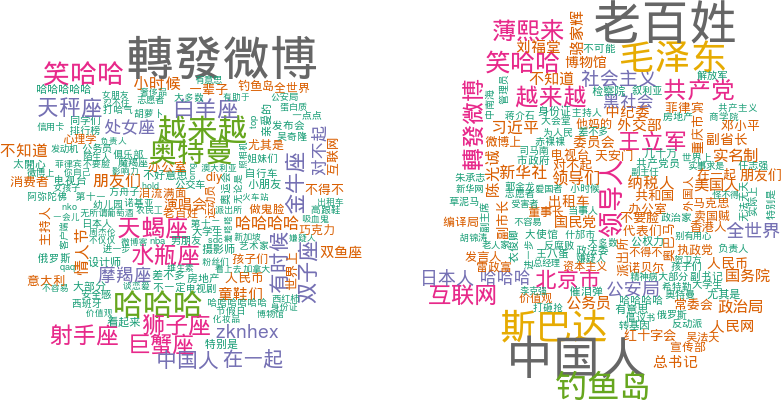
\includegraphics[scale = 0.65]{wc.png}
  \caption{Noncensored (Left) and Censored (Right) Tweets Word Cloud}
  \label{fig:wordcloud}
\end{figure*}

Figure~\ref{fig:wordcloud} shows the word clouds for the noncensored tweets (left) and for the censored tweets (right). Some terms are found often in both sets, namely 轉發微博 (retweet), 哈哈 (haha), 中国人 (Chinese people), and 越来越 (more and more). 

However, censored tweets tend to be much more political. 钓鱼岛 (Diaoyu Islands) refer to the disputed island chains. 斯巴达 (Sparta) is actually a play on the fact that Sparta in Chinese (sibada) is nearly a homophone for 十八大 (shibada), the 18th National Party Congress where the previous president Hu Jintao stepped down and the current president -- Xi Jinping -- took his place.\footnote{Chinese internet users often rely on homophone tricks such as these to evade automatic keyword censoring. In this case, we can see that it was not 100\% effective.} There tend to be more people names in the censored tweets, such as 毛泽东 (Mao Zedong, former chairman of the Chinese Communist Party), 薄熙来 (Bo Xilai, disgraced Chongqing party chief), 王立军 (Wang Lijun, vice-mayor of Chongqing under Bo), and others. There are also references to the Chinese government, such as 领导人 (leadership) and 共产党 (Communist Party), and the masses (老百姓).

In comparison, the noncensored tweets appear much more benign. One of the most common terms is 奥特曼, which refers to the fictional Japanese superhero Ultraman, who is apparently quite popular among a certain generation in China. Many popular terms are simply astrology zodiac signs e.g. Leo (狮子座), Sagittarius (射手座), etc. The astrology most likely comes from a bot or person that tweets horoscopes every day.\footnote{Astrology is actually fairly \href{https://newrepublic.com/article/119500/chinese-astrology-surprising-prominence-horoscopes}{popular in China}.} The popularity of the term Ultraman can perhaps be attributed to the creation of a noodle-robot that looked \href{http://asiasociety.org/blog/asia/video-when-going-gets-tough-superhero-robot-turns-noodle-making}{like Ultraman in 2012}. The conclusion would be that we should look for more overtly political words to classify censored tweets.

For the assignment, we kept all the censored tweets but kept only a small subsample (0.1\%) of the noncensored tweets. Noncensored tweets were randomly sampled from the entire dataset such that the number of noncensored tweets would be roughly twice that as the number of censored tweets within our data.\footnote{There was no particular reason that this ratio was chosen.} Whereas 0.03\% of tweets are censored in the entire dataset, 34\% of tweets are censored in our small subsample. The training set was constructed such that half of the tweets would be censored while the other half would be noncensored. The validation and test sets were deliberately constructed to look like one another. 

\begin{table*}
  \centering
  \begin{tabular}{|l|c|c|c|c|}
    \hline
    Statistic & Training Set & Validation Set & Test Set & Total \\
    \hline
    Retweets & 47930 & 41285 & 41414 & 130629 \\
    Unique Users & 39719 & 50446 & 50620 & 107907 \\
    \hline
    Censored Tweets & 43042 (50\%) & 21521 (25\%) & 21521 (25\%) & 86084 (34\%)  \\
    Non-censored Tweets & 43042 (50\%) & 63291 (75\%) & 63292 (75\% )& 169625 (66\%) \\
    Total Tweets & 86084 & 84812 & 84813 & 255709 \\
    \hline
  \end{tabular}
  \caption{Dataset Statistics}
  \label{tab:descript}
\end{table*}

Table~\ref{tab:descript} shows some descriptive statistics for our dataset. It appears that more than half of the tweets in our subsample are retweets.\footnote{Note that this is a function of how the original dataset was constructed. This is not an artifact of our random sampling strategy.} We also see that, on average, each user is producing 2.5 tweets in our dataset. This implies that many tweets are correlated with one another. A retweet is very likely related to whatever the original tweet was, and individual users will probably tweet similar things over time. These aspects of the data will be incorporated into our features as described in Section~\ref{sec:pred}.

\begin{figure}
  \centering
  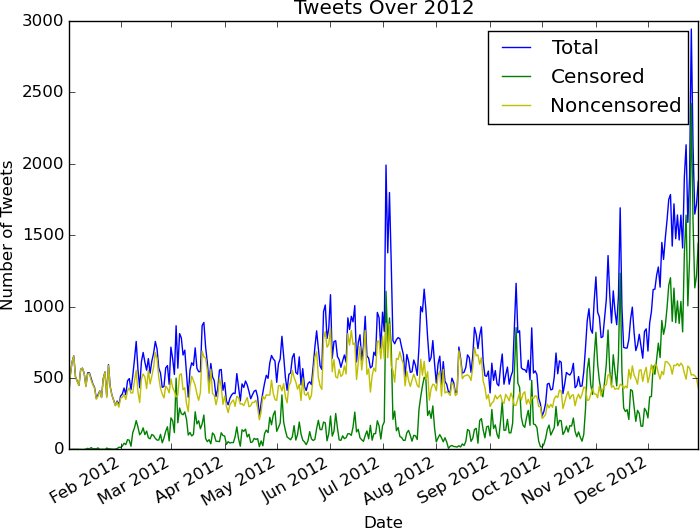
\includegraphics[scale=0.5]{tweetTime.png}
  \caption{Tweets over Time}
  \label{fig:ts}
\end{figure}

Figure~\ref{fig:ts} shows the distribution of tweets over time in our small subsample. While the number of noncensored tweets is somewhat constant over time, the number of censored tweets clearly vary greatly over time. There are few censored tweets in the beginning of the year, with a spike coming in mid-2012 and a huge increase near the end of 2012. The spike at the end corresponds to the 18th Party Congress mentioned above. The spike in the summer of 2012 roughly corresponds to anti-Japanese protests held in multiple Chinese cities. A good predictive model should therefore require some way to account for the temporal aspect of censorship. 

In other words, there are many factors at play in determining whether a tweet is censored or not. How we explicitly model these factors will be explained in the following section.

\section{Predictive Task} \label{sec:pred}
We would like to predict which tweets are censored in this dataset i.e. a binary-class prediction. To evaluate our model, we will simply use classification accuracy -- the proportion of tweets that are labelled correctly. If we were Chinese government censors, then perhaps we would evaluate recall or $F_\beta$ instead.\footnote{Recall that $F_\beta = (1+\beta^2) \cdot \frac{\text{precision} \cdot \text{recall}}{\beta^2 \text{precision} + \text{recall}}$} The idea is that a government censor would prefer flagging a ``harmless'' tweet for censorship over accidentally letting a ``harmful'' tweet through. We are [fortunately] not Chinese government censors, so we will stick with evaluating our model using classification accuracy. 

Our data are split into training, validation, and test sets using the procedure described in Section~\ref{sec:pred}. We purposely oversampled censored tweets (by including literally all of them) in our training, validation, and test sets. This oversampling makes sense for the training set, since we want a balanced sample to be used for training the model. This also certainly made the predictive task easier, since a trivial predictor -- one that predicts no tweets are censored -- on the entire dataset would have been 99.97\% accurate while only 75\% accurate on our test set. 

The features we chose to include in our model can be categorized into two types: the actual text of the tweet and metadata about the tweet. For the text, we either used a simple bag-of-words representation with term frequency-inverse document frequency (tf-idf) weighting or a latent Dirichlet allocation (LDA) topic model to represent each tweet. 

Processing Chinese text data is not exactly the same as processing English text. One of the major differences is that there are no spaces in Chinese text, so spaces must first be inserted between words in each document before a bag-of-words representation can be made. This process is known as segmentation. 

Another major difference between Chinese and English is that Chinese is a ideogram-based language while English is an alphabet-based language. This creates problems for determining where to insert spaces. Consider the following example. The word 電 means electricity, and the word 腦 means brain. However, combining the two words yields 電腦, which means computer.

The segmentation task therefore becomes a machine learning problem where the model tries to predict what type of $n$-gram a word is. When the segmenter encounters a word like 電腦, it must decide whether this is a bigram (computer) or two unigrams (electric brain). We had our hands full with our actual predictive task, so we used the basic Chinese segmenter provided in the \href{http://nlp.stanford.edu/software/segmenter.shtml}{Stanford Word Segmenter} \cite{Chang2008}. After segmentation, we removed punctuation and numbers.

The easiest baseline to beat would be the trivial predictor that predcts that every tweet is not censored. This would result in 50\% error on our training

\section{Model}
\begin{figure}
  \centering
  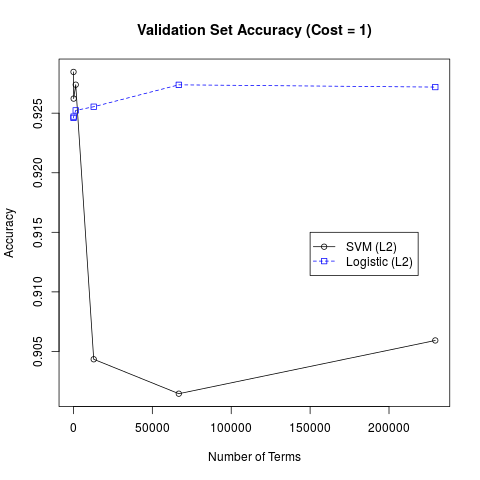
\includegraphics[scale=0.5]{valid_numTerms.png}
  \caption{Sparsity Tuning}
  \label{fig:sparse}
\end{figure}

When the bag-of-words representation for text was initially created, it contained 229,334 terms. We hypothesize that many of these terms might be completely useless or even detrimental to the model by inducing overfitting. We therefore attempted some dimension reduction via just dropping infrequent terms and by applying LDA (discussed later). Infrequent terms were removed based on their sparsity, using maximum allowed sparseness values of 0.99, 0.995, 0.999, 0.9999, 0.99999, and 1 (all terms included). These correspond to 48, 141, 1451, 12849, 66771, and 229334 terms, respectively. Figure~\ref{fig:sparse} shows the results from tuning the number of terms to include in the basic bag-of-words representation of tweets. 

Indeed, there is a small reduction in error on the validation set when we reduce the number of terms. The accuracy for SVM is maximized when we include 1,451 terms instead of the full 229,334 terms. The accuracy for logistic regression is maximized when we have 12,849 terms.



\begin{figure}
  \centering
  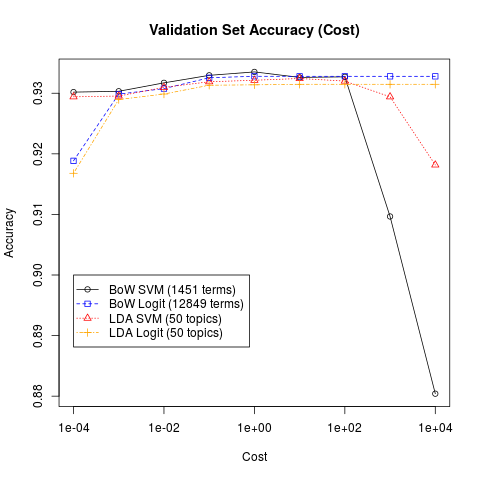
\includegraphics[scale=0.5]{valid_cost.png}
  \caption{Cost Tuning}
  \label{fig:cost}
\end{figure}

The results from tuning the cost parameters are shown in Figure~\ref{fig:cost}.
\section{Literature}

\section{Results}

\bibliographystyle{abbrv}
\bibliography{writeup}
\end{document}
